\documentclass[english]{presentation}
%\setbeameroption{show notes on second screen}
%\setbeameroption{show only notes}

\usepackage{chngpage}
\usepackage{array}
\usepackage{xcolor}

% beamer style file
\usepackage{presento}

\usepackage{textpos}
\setlength{\TPHorizModule}{1cm}
\setlength{\TPVertModule}{1cm}

\usepackage{stmaryrd}
\usepackage{scalerel}

% strikethrough text
\usepackage[normalem]{ulem}

% macros
\usepackage{mama}
\usepackage{opengames}

\addbibresource{./bibliography.bib}

\title{\bfseries Translating Extensive Form Games\\to Open Games with Agency}
\subtitle{ACT2021}
\institute{Mathematically Structured Programming group,\\Department of Computer and Information Sciences,\\University of Strathclyde}
\author{\underline{Matteo Capucci}, Neil Ghani,\\Jérémy Ledent, Fredrik Nordvall Forsberg}
\date{\vfill July 14th, 2021}

\begin{document}
	\begin{frame}[plain]
		\maketitle
	\end{frame}

	\begin{frame}{Introduction}
	\vfill
	\begin{quotation}
		\centering
		Game theory is the mathematical study of interaction\\
		among independent, self-interested agents.\\
		{\color{colornote}-- Essentials of Game Theory, \cite{leyton2008essentials}}
	\end{quotation}

	\vfill
	\textbf{Examples}: economic and ecological games, machine learning, etc. \textcolor{colornote}{$\rightsquigarrow$ \emph{cybernetics}.}

	\vfill
	% ugh
	\onslide<2->{
		\alt<3>{
			Open games as a framework for compositional game theory

			\begin{center}
				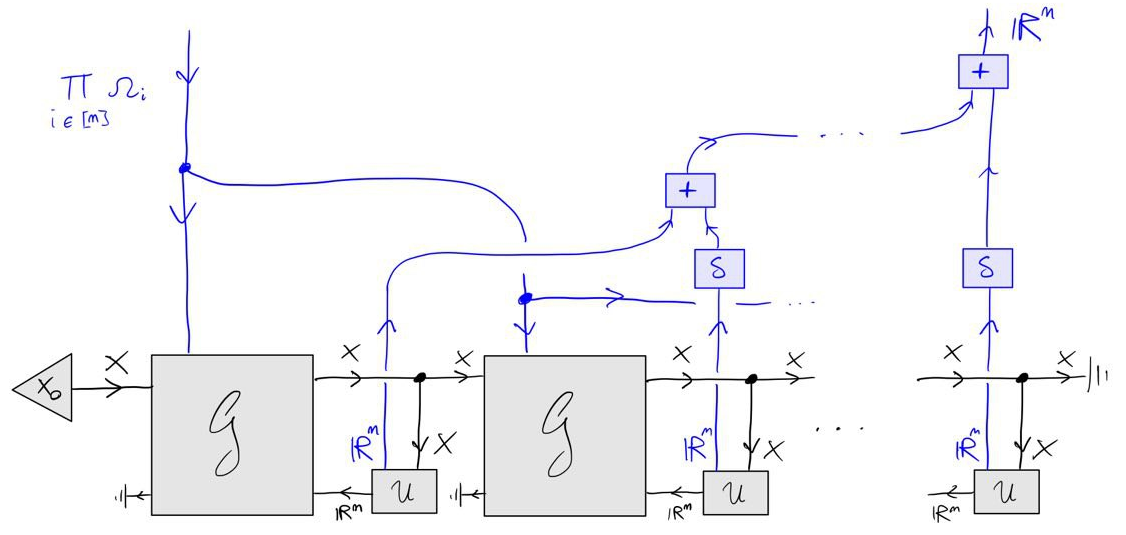
\includegraphics[width=.8\textwidth]{figures/og_ex.png}
			\end{center}

			Shows causality without being too unwieldy, compositional (\textcolor{coloraccent}{$\rightsquigarrow$ large scale}).\\
			Also: string diagrams are nice to work with!
		}{
			Classical game theory: \textbf{normal form} and \textbf{extensive form}

			\begin{center}
				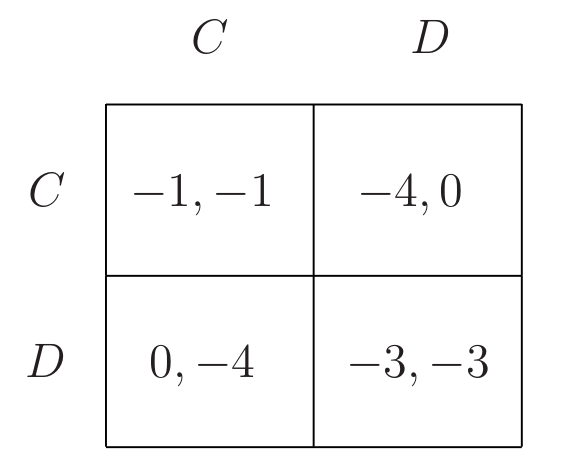
\includegraphics[width=.34\textwidth]{figures/pd_norm.png}
				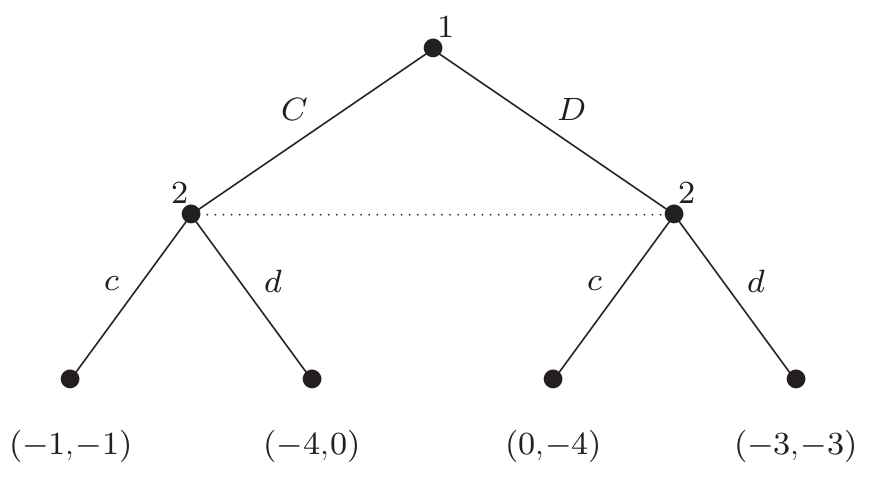
\includegraphics[width=.5\textwidth]{figures/pd_ext.png}
			\end{center}

			\textbf{Drawbacks}: too little information (NF), too much information (EF), unclear causal relationships (both). Most importantly: non-compositional! (\textcolor{coloraccent}{$\rightsquigarrow$ small scale})
		}
	}
\end{frame}

\begin{frame}{Introduction}
	Translating NF to open games is 'trivial' (there's only a utility function)...

	\begin{center}
		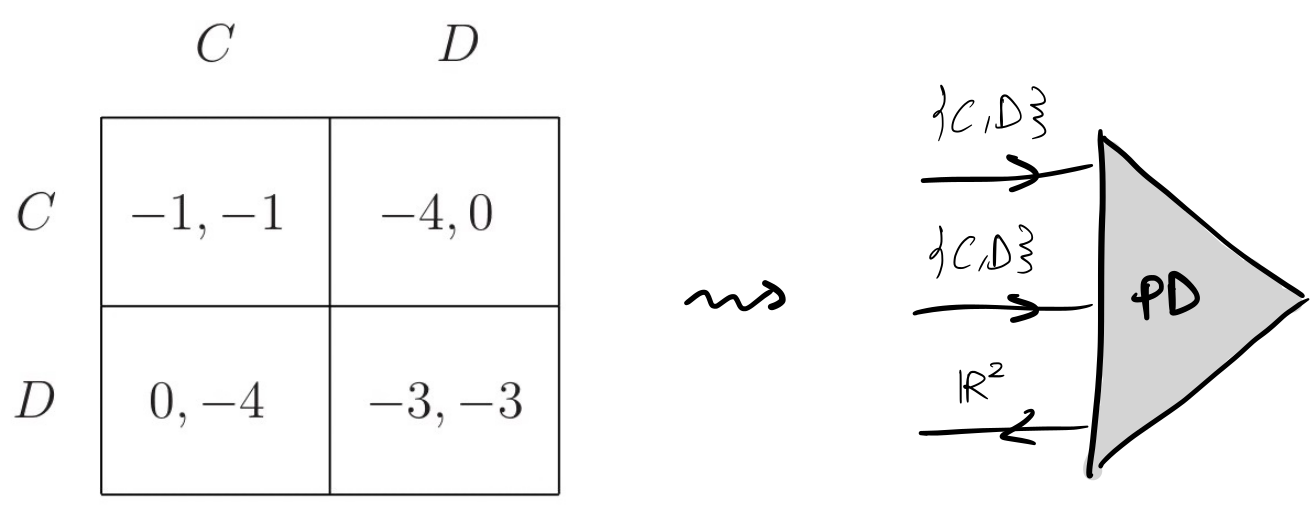
\includegraphics[width=.7\textwidth]{figures/nf_to_og.png}
	\end{center}

	\onslide<2->{
		Translating EF to open games (mantaining a similar causal structure) is non-trivial:
		\begin{enumerate}
			\item EF is a \textbf{non-inductive definition}, and it's messy to map a whole tree in one go.
			\item Open games don't have an \textbf{explicit notion of players}, necessary to model imperfect information and to correctly compute equilibria.
		\end{enumerate}
	}
	\onslide<3->{
		To do so, we introduce:

		\begin{enumerate}
			\item Open games with \textbf{agency}, an improved compositional framework for games,
			\item An operator calculus for games, in particular new \textbf{choice operators},
			\item \textbf{Inductive data types for EF trees} with (im)perfect information.
		\end{enumerate}
	}
\end{frame}

% 1. Open Games with Agency
% - lenses and bidirectional information flow (= attuale)
% - straight to: arena as parametrised lens (slide 12 ma con strat (slide 23 but rename costrategies and redraw))
% - composition
% - choice
% - reparametrisation & regrouping
% - closing an arena: state and payoff
% - keep slide 18
% - keep slide 22-25 but (a) condense intro to 1 slide, (b) slide 25 on directly exemplify lens_S (or not?)
% - slide 27 add '\in \varepsilon \boxtimes \eta(k)' to the diagram
% - put slide 28 in slide 29 with def

% 2. Extensive form and translation
% - lots of pictures of trees
% - PETree & defs
% - translation: a single picture
% - an example (probably to work out 'live'?)
% - IETree & defs
% - translation: a single picture
% - an example (probably to work out 'live'?)

% 3. Future work
% - Functoriality?
% - Copy from paper

	\begin{framecard}
	{\color{colorbg}
	\bfseries

	\hugetext{Open games with agency}}
\end{framecard}

\begin{frame}{What is a game?}
	\begin{quotation}
		\centering
		Game theory is the mathematical study of {\color<2->{colorarena}interaction}\\ among independent, self-interested {\color<2->{coloragents}agents}.\\
		{\color{colornote}-- Essentials of Game Theory, \cite{leyton2008essentials}}
	\end{quotation}

	\vfill
	\begin{center}
		\alt<2->{
			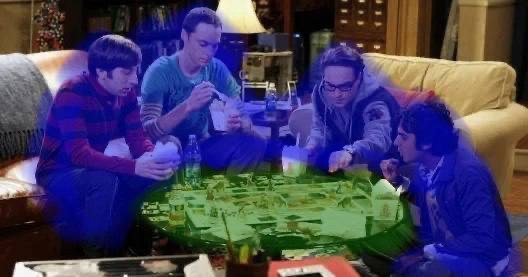
\includegraphics[width=.5\textwidth]{figures/board_games2.jpg}
		}{
			
\includegraphics[width=.5\textwidth]{figures/board-games.png}
		}
	\end{center}

	\vfill
	\onslide<2->{
		A game factors in two parts:
		\begin{enumerate}
			\item An \textcolor{colorarena}{\textbf{arena}}, which models the \textbf{dynamics} of the game.
			\item \textcolor{coloragents}{\textbf{Players}}, which intervene in the arena by making \textbf{decisions} at different points.
		\end{enumerate}
	}

	\vfill
	\onslide<3->{
		A \textcolor{coloragents}{strategy} $\colag{\omega \in \Omega_p}$ for a player $\colag{1 \leq p \leq N}$ is a policy $\colag p$ uses to make their decisions (e.g. a choice of move for each of $\colag p$'s rounds).

		\vfill
		A \textcolor{coloragents}{strategy profile} is a strategy for each player $\colag{\Omega = \Omega_1 \times \cdots \times \Omega_N}$.
	}
\end{frame}

\begin{frame}{What is an arena?}
	\begin{center}
		An \textcolor{colorarena}{arena} is an open system with three boundaries:
	\end{center}

	{\issue change strategies to profiles}
	\begin{center}
		\includegraphics[clip, page=2, trim=0cm 3cm 3cm 2cm, width=.8\textwidth]{figures/drawings.pdf}
	\end{center}

	This is a \textbf{parametrised lens} $\textcolor{colorarena}{\A : (X,S) \nlongto{\textcolor{coloragents}{(\Omega, \Comega)}} (Y,R)}$ specified by two maps
	\begin{eqalign*}
		\textcolor{colorarena}{\play} &: \textcolor{coloragents}{\Omega} \textcolor{colorarena}{\times X \to Y},\\
		\textcolor{colorarena}{\coplay} &: \textcolor{coloragents}{\Omega} \textcolor{colorarena}{\times X \times R \to \textcolor{coloragents}{\Comega} \times S}
	\end{eqalign*}
	\textcolor{colornote}{See~\cite{capucci2021towards},~\cite{backprop}.}
\end{frame}

\begin{frame}{What is an arena?}
	\begin{center}
		It can be `closed' by specifying an \textcolor{colorarena}{\textbf{initial state}} and a \textcolor{colorarena}{\textbf{utility function}}:
	\end{center}

	\begin{center}
		\includegraphics[clip, page=4, trim=4.5cm 3cm 2cm 7cm, width=.9\textwidth]{figures/drawings.pdf}
	\end{center}
	Observe that $\colar{\Lens(1,1)(X,S) \iso X}$ and $\colar{\Lens(Y,R)(1,1) \iso Y \to R}$.
\end{frame}

\begin{frame}{What is an arena?}
	\begin{center}
		A \textcolor{colorarena}{\textbf{closed arena}} amounts to an evaluation of strategies with rewards:
	\end{center}

	\vspace{5ex}
	\begin{center}
		\includegraphics[clip, page=5, trim=3cm 6.5cm .5cm 5cm, width=.9\textwidth]{figures/drawings.pdf}
	\end{center}
\end{frame}

\begin{frame}{What are players?}
	\begin{center}
		\textcolor{coloragents}{Players} are a \emph{distinct part} of the game (seen as a \textbf{system})\\
		which expresses \textcolor{coloragents}{preferences} by means of a \textcolor{coloragents}{\textbf{selection function}}:
	\end{center}

	{\fontsize{1.5em}{1.5em}\selectfont
	\begin{equation*}
		\colag{\varepsilon} : (\colar{\colag{\Omega} \to \colag{\Comega}}) \longto \copow{\colag \Omega}
	\end{equation*}
	}

	In a single-player game, typically $\colag\Omega$ is `finite', $\colag{\Comega = \R}$ and $\colag\varepsilon$ is $\argmax$:
	\begin{equation*}
		\colag{\argmax(\colar{u : \colag\Omega \to \colag\R})} = \{\colag{\omega \in \Omega} \suchthat \text{$\colag\omega$ maximises $\colar u$}\} \subseteq \colag\Omega.
	\end{equation*}
\end{frame}

% a player observes how other players chose to play in the game (i.e. their strategies), but their only leverage is to change their own strategy.
% a Nash equilibrium is a stand-off situation: nobody can change strategy without getting worse outcomes _given the other players do not deviate_
% notice this doesn't mean that, as a group, players realize their optimal outcome, which might require players to cooperate and deviate jointly
\begin{frame}{What is a Nash equilibrium?}
	\begin{center}
		A strategy profile is a \textbf{Nash equilibrium}\\
		if no player has incentive to \emph{unilaterally} change strategy.
	\end{center}

	\vfill
	\begin{center}
		
\includegraphics[width=.7\textwidth]{figures/nash.png}
	\end{center}

	\vfill
	\textcolor{colornote}{Traditionally `the' goal of game theory is determining Nash equilibria of games, though this is not necessarily the case anymore (see: \cite{fudenberg1998theory}).}
\end{frame}

\newcommand{\altunderbrace}[3]{\alt<#1->{\underbrace{#2}_{#3}}{#2}}
\newcommand{\altoverbrace}[3]{\alt<#1->{\overbrace{#2}^{#3}}{#2}}

\begin{frame}{What is a Nash equilibrium?}
	The assignment $\colag{\S(\Omega,\Comega)} := (\colar{\colag{\Omega} \to \colag{\Comega}}) \longto \copow{\colag \Omega}$ is functorial on $\Lens$.

	\vfill
	Crucially, $\colag\S$ admits a lax monoidal structure we call \textbf{Nash product}:
	\begin{eqalign*}
		&\colag{- \boxtimes -} : \colag{\S(\Omega_1,\Comega_1)} \times \colag{\S(\Omega_2, \Comega_2)} \longto \colag{\S(\Omega_1 \times \Omega_2, \Comega_1 \times \Comega_2)}\\[1ex]
		&\colag{(\varepsilon \boxtimes \eta)}(\colar{u}) = \{ \colag{(\omega_1,\omega_2)} \suchthat \colag{\omega_1} \in \colag{\varepsilon}(\colar{u_1(-,\colag{\omega_2})})\ \text{and}\ \colag{\omega_2} \in \colag{\eta}(\colar{u_2(\colag{\omega_1}, -)})\}\\
		&\phantom{\colag{(\varepsilon \boxtimes \eta)}(\colar{u})}\onslide<2->{ = \textcolor{coloraccent}{\text{profiles s.t. `no agent wants to unilaterally deviate'}}}
	\end{eqalign*}
	where $\colar{u = (u_1,u_2) : \colag{\Omega_1} \times \colag{\Omega_2} \to \colag{\Comega_1} \times \colag{\Comega_2}}$.

	\vfill
	\onslide<3->{
		Hence if we have players $\colag{P = \{1, \ldots, N\}}$, each with preferences $\colag{\varepsilon_i \in \S(\Omega_i, \Comega_i)}$, we get:
		\begin{equation*}
			\colag{\varepsilon_1 \boxtimes \cdots \boxtimes \varepsilon_N} : (\altoverbrace{5}{\altunderbrace{4}{\colar{\colag{\Omega_1 \times \cdots \times \Omega_N}}}{\colag{\text{strat. profiles}}} \;\colar{\longto}\; \altunderbrace{4}{\colag{\Comega_1 \times \cdots \times \Comega_N}}{\colag{\text{reward vectors}}}}{\colar{\text{utility functions/\textbf{closed arenas}}}}) \longto \altunderbrace{6}{\copow{(\colag{\Omega_1 \times \cdots \times \Omega_N})}}{\textcolor{coloraccent}{\text{Nash equilibria}}}
		\end{equation*}
	}
\end{frame}

% \begin{frame}{Interlude: selection functions}
% 	Let $\S(X,S) := (X \to S) \to \pow{X}$. This is a functor on lenses:
% 	\begin{eqalign*}
% 		\S(\alpha) : \S(X,S) &\longto \S(Y,R)\\
% 		\varepsilon &\longmapsto \lambda k \,.\, \{x \cmp \alpha \suchthat x \in \varepsilon(\alpha \cmp k)\}
% 	\end{eqalign*}
% 	where $\alpha : (X, S) \to (Y,R)$ and we implicitly used $\Lens((1,1),(Y,R)) \iso Y \to R$ and $\Lens((X,S),(1,1)) \iso X$:

% 	(drawing)

% 	This functor is lax monoidal (\textbf{Nash product}):
% 	\begin{eqalign*}
% 		- \boxtimes - : \S(X,S) \times \S(Y,R) &\longto \S(X \times Y, S \times R)\\
% 		(\varepsilon, \eta) &\longmapsto \lambda k \,.\, \{ (x,y) \suchthat x \in \varepsilon(k_1(x,y))\ \text{and}\ y \in \eta(k_2(x,y))\}
% 	\end{eqalign*}
% 	(drawing)

% 	\textcolor{colornote}{This yields a moncat $\Lens_\S = \underset{mon}\int \S$.}
% \end{frame}

\begin{frame}{The definition}
	\begin{definition}
		An \textbf{open game with agency} is a pair
		\begin{equation*}
			\G \quad = \quad (\ \colar{\A : (X,S) \nlongto{\colag{(\Omega, \Comega)}} (Y,R)}, \quad \colag{\varepsilon  : \S(\Omega, \Comega)}\ )
		\end{equation*}
		whose equilibria are given by
		\begin{equation*}
			\eq_\G(x, k) = \colag{\varepsilon(}\colar{x \cmp \A \cmp k}\colag{)}.
		\end{equation*}%
		\textcolor{colornote}{In this way we recover the equilibrium predicate of open games (\cite{ghani2018compositional}).}
	\end{definition}

	\vfill
	\onslide<2->{
		\begin{definition}
			$\G$ \textbf{has set of players $\colag P$} when
			\begin{equation*}
				\colag{
					\Omega = \prod_{p \in P} \Omega_p, \quad \Comega = \prod_{p \in P} \Comega_p, \quad \varepsilon = \Boxtimes_{p \in P} \varepsilon_p
				}
			\end{equation*}
			in which case
			\begin{equation*}
				\eq_\G(x, k) = \colag{(\Boxtimes_{p \in P} \varepsilon_p)(}\colar{x \cmp \A \cmp k}\colag{)}.
			\end{equation*}
		\end{definition}
	}
	%where $(-)^\top : \Lens_{(\Omega, \Comega)}((1,1),(1,1))\ \iso\ \Omega \to \Comega$.
\end{frame}

% Let's focus on arenas, aka parametrised lenses, for a while...
\begin{frame}{Composing games}
	%\textcolor{colorarena}{Arenas} are the compositional heart of open games with agency:

	\begin{itemize}
		\item \textbf{Sequential composition}
		\begin{center}
			\includegraphics[clip, page=7, trim=2.5cm 21cm 1.5cm 1cm, width=.9\textwidth]{figures/drawings.pdf}
		\end{center}
		\item \textbf{Parallel composition}
		\begin{center}
			\includegraphics[clip, page=7, trim=2cm 5cm 1cm 13cm, width=.9\textwidth]{figures/drawings.pdf}
		\end{center}
	\end{itemize}

	\textbf{Notice}: these operators \underline{can} be extended to games:
	\begin{equation*}
		(\colar{\A_1}, \colag\varepsilon) \cmp (\colar{\A_2}, \colag\eta) := (\colar{\A_1 \cmp \A_2}, \colag{\varepsilon \boxtimes \eta}), \quad (\colar{\A_1}, \colag\varepsilon) \otimes (\colar{\A_2}, \colag\eta) := (\colar{\A_1 \otimes \A_2}, \colag{\varepsilon \boxtimes \eta})
	\end{equation*}
\end{frame}

\begin{frame}{Composing arenas}

	\begin{itemize}
		\item \textbf{External choice}
		\begin{center}
			\includegraphics[clip, page=8, trim=0 17cm 2cm 4cm, width=.9\textwidth]{figures/drawings.pdf}
		\end{center}
		The `environment' chooses which game to play, agents are prepared to play both.
		\item \textbf{Internal choice}
		\begin{center}
			\includegraphics[clip, page=8, trim=1.5cm 7cm 2cm 14cm, width=.9\textwidth]{figures/drawings.pdf}
		\end{center}
		The `environment' can play either game, agents choose which one.
	\end{itemize}

	\textbf{Notice}: these operators \underline{can't} be extended to selection functions in a canonical way! \textcolor{colornote}{(Actually $\oplus$ \underline{can} if we refine our typing judgments)}
\end{frame}

\begin{frame}{Reparametrisation}
	Most importantly arenas form a (locally fibred) bicategory: one can \textbf{reparametrise} along a lens $\colag{\alpha : (\Omega', \Comega') \to (\Omega, \Comega)}$.

	\vfill
	\begin{center}
		\includegraphics[clip, page=9, trim=0cm 19cm 13cm 0cm, width=.9\textwidth]{figures/drawings.pdf}
	\end{center}

	\vfill
	This is crucial for introducing agency!

	\vfill
	Lenses in the blue direction represent `\textcolor{coloragents}{players dynamics}', e.g. voting, observational constraints, reward distributions (imputation), ...
	%\vfill
	%\textcolor{colornote}{If we work in $\Para_{\times_\S}(\Lens_\S)$, we see that `$(1,1,\top)$ coclassifies equilibria', i.e. $(1,1,\top) \twoto \G \iso \eq_\G$.}
\end{frame}

\begin{frame}{Regrouping}
	If $\colar\A$ has set of players $\colag P$ and $\colag{r : P \to Q}$ is a function, we can turn $\colar\A$ into an arena with players $\colag Q$ by reparametrising along the permutation of $\colag{\prod_{p \in P} \Omega_P}$ induced by $\colag r$:
	\begin{equation*}
		\colag{\regroup_r : ({\textstyle\prod}_{q \in Q} (r^* \Omega)_q, {\textstyle\prod}_{q \in Q} (r^* \Comega)_q) \longto ({\textstyle\prod}_{p \in P} \Omega_p, {\textstyle\prod}_{p \in P} \Comega_p)}
	\end{equation*}
	\begin{example}<2->
		If $\colar{\A_1}$ and $\colar{\A_2}$ have the same players $\colag{P = \{1,2\}}$, $\colar{\A_1 \cmp \A_2}$ has players $\colag{P+P}$. Regrouping along $\colag{\nabla : P+P \to P}$ restores the correct set of players.
		\begin{center}
			\only<-2>{
				\includegraphics[clip, page=10, trim=0cm 24.5cm 25.7cm .5cm, width=.7\textwidth]{figures/drawings.pdf}
			}
			\only<3>{
				\includegraphics[clip, page=10, trim=18cm 13cm 7cm 6.6cm, width=.7\textwidth]{figures/drawings.pdf}
			}
			\only<4>{
				\includegraphics[clip, page=10, trim=0cm 13cm 25cm 7cm, width=.7\textwidth]{figures/drawings.pdf}
			}
			\only<5>{
				\includegraphics[clip, page=10, trim=.5cm 2.2cm 25cm 17.5cm, width=.7\textwidth]{figures/drawings.pdf}
			}
		\end{center}
	\end{example}
\end{frame}

\begin{frame}{Tying}
	By reparametrising along $\colag{(\Delta, \mathsf{combine})}$ (where $\colag{\mathsf{combine} = +, \pi_2, \max, \ldots}$), we can enforce the same strategies to be played at different points of a game.

	\begin{example}<2->
		Repeated games: play the same strategies at every round
		\begin{center}
			\includegraphics[clip, page=11, trim=0cm 15cm 10cm 0cm, width=.85\textwidth]{figures/drawings.pdf}
		\end{center}
	\end{example}

	\vfill
	\onslide<3->{
		\textbf{Notice}: $\colag{(\Delta, \mathsf{combine})^*}\colar{(\A_1 \cmp \A_2)}$ lies outside the image of $\cmp$/$\otimes$/$\oplus$/$\&$, hence introduces 'non-compositional' effects $\rightsquigarrow$ \textbf{`\textcolor{coloragents}{agency} is non-local'.}
	}
	%\textcolor{colornote}{We'll use this soon to treat imperfect information. Also useful for Markov games.}
\end{frame}

	\begin{framecard}
	{\color{colorbg}
	\bfseries

	\hugetext{Extensive form games\\\& their translation}}
\end{framecard}

\begin{frame}{Extensive form}
	Extensive form is a classical formalism for games:

	(nice pic)

	A game is presented as a (rooted) tree, which should reflect the possible unfoldings of the game.
	Each node is labelled with a \emph{player}. Branches represent possible \emph{moves} and \emph{payoff vectors} await at the leaves.

	Two kinds:
	\begin{enumerate}
		\item Perfect information: any player always knows exactly the state of the game (path from root to their nodes)
		\item Imperfect information: otherwise
	\end{enumerate}

	{\color{colornote}As customary in classical game theory, all players $\argmax$ their payoff.}
\end{frame}

\begin{frame}{PETs as inductive type}
	We can easily represent PETs with an inductive type:

	(inductive type)

	where $P : \Set$ are players, $R : \Set$ are rewards.

	(tree and corresponding term)
\end{frame}

\begin{frame}{PETs}
	Correspondigly, we can define what strategies/moves/states/utilities are with inductive definitions:

	(def)
\end{frame}

\begin{frame}{Translation}
	Finally, we can translate any PETree to an open game:

	(pic)

	where
	\begin{enumerate}
		\item $\Dec{[n]}{R^P}$ is the `trivial' game where moves = strategies = $[n]$ and coplay is just $\Delta$.
		\item $\regroup_p$ is regrouping along $\{p\} + P \to P$.
	\end{enumerate}
\end{frame}

\begin{frame}{IETs}
	Imperfect information extensive form games are decorated with \emph{information sets}:

	(pic)

	Nodes in the same information set cannot be distinguished by players. Players do not share information sets, each player has their own partition of their nodes in information sets. Nodes in the same information set have the same moves.

	Limit case: all information sets are singleton = perfect information.
\end{frame}

\begin{frame}{IETs as inductive type}
	We can also represent IETs with an inductive type:

	(inductive type)

	where $P : \Set$ are players, $R : \Set$ are rewards, $I : \Set$ is a set of information labels, $\belongs : I \to P$ assigns information sets to players, $n : I \to \N^+$ assigns uniformly moves to nodes of the same information set.

	(tree and corresponding term)
\end{frame}

	\begin{frame}{Conclusions}
	In this work:
	\begin{enumerate}
		\item We have seen how games naturally decompose in \emph{arenas} and \emph{selection functions}, with \emph{reparametrisations} playing a key role
		\item This allows to handle long-range correlations in players' behaviour
		\item Hence we can easily map extensive form trees to open games with agency
	\end{enumerate}
\end{frame}

\begin{frame}{Future directions}
	\begin{enumerate}
		\item Is the translation `functorial'? Possible domain cat described in \cite{streufert2021category}.
		\item Once the diagram is drawn, can we simplify it using topological moves?
		e.g. mapping `simultaneity' to $\otimes$.
		\item Infinite trees?
		\item Can we treat SPE?
		\item What kind of assignment is $\colag{\argmax} : \colar{\Arenas} \to \Games$?
		\item Can we make selections compositional?
		\item Dependent types
	\end{enumerate}
\end{frame}


	\begin{framecard}
		{\color{colorbg}
		\bfseries

		\hugetext{Thanks for your attention!}\\
		\vfill
		\largetext{Questions?}}
	\end{framecard}

	\begin{frame}[allowframebreaks]{References}
		\nocite{*}
		\printbibliography
	\end{frame}
\end{document}
